% LaTeX source for ``Algorithms for Computer Simulation of Molecular Systems''
% Copyright (c) 2023 รังสิมันต์ เกษแก้ว (Rangsiman Ketkaew).

% License: Creative Commons Attribution-NonCommercial-NoDerivatives 4.0 International (CC BY-NC-ND 4.0)
% https://creativecommons.org/licenses/by-nc-nd/4.0/

\chapter{การพัฒนาซอฟต์แวร์สำหรับเคมีเชิงคำนวณ}
\label{ch:software_dev}

%----------------------------------------
\section{การเขียนโปรแกรมทางเคมีเชิงคำนวณ}
%----------------------------------------

ถ้าหากผู้อ่านอยากจะศึกษาการเขียนโปรแกรมทางเคมีเชิงคำนวณจะเริ่มยังไงดี เช่น ต้องการเขียนโปรแกรม Density Functional Theory (DFT) 
หรือ Implement วิธีโครงสร้างเชิงอิเล็กทรอนิกส์ (Electronic Structure) ผมขอให้ความเห็นอย่างนี้ครับว่าการจะที่เขียนโปรแกรมทางเคมี%
คำนวณขึ้นมาสักโปรแกรมหนึ่งนั้นใช้เวลามากพอสมควรเพราะว่ามีรายละเอียดที่ซับซ้อนมาก (เวลาที่ใช้ในการเขียนนั้นขึ้นอยู่กับว่าเขียนคนเดียวหรือช่วย%
กันเขียนหลายคน) ดังนั้นผมแนะนำว่าสำหรับผู้ที่เพิ่งเริ่มต้นการเขียนโปรแกรมทางวิทยาศาสตร์ควรศึกษาจากโปรแกรมมาตรฐานที่ได้รับความนิยมอยู่แล้ว 
ผมไม่ได้บอกว่าห้ามเขียนโปรแกรมใหม่เองแบบเริ่มจากศูนย์หรือ From Scratch แต่ถ้าหากว่าเราเริ่มต้นเรียนรู้จากโปรแกรมที่ได้รับความนิยมและใช้งาน%
กันอย่างแพร่หลายอยู่แล้วก็มีข้อดีดังนี้ 

\begin{itemize}
    \item ประหยัดเวลา ไม่ต้องมานั่งศึกษาหรือเขียนโค้ดใหม่เองทั้งหมด
    
    \item ได้เรียนรู้วิธีการเขียนโค้ดที่มีประสิทธิภาพจากนักพัฒนาคนอื่น ๆ 
    
    \item เป็นการต่อยอดและพัฒนาโปรแกรมนั้น ๆ ให้ดีขึ้นไปอีกเพราะเราไม่จำเป็นต้องมา Reinvent the Wheel 
    
    \item เป็นการสร้างเครือข่ายนักวิจัยและความร่วมมือทางวิชาการในระดับนานาชาติ 
\end{itemize}

\noindent อย่างไรก็ตามถ้าหากใครอยากจะเริ่มเขียนโปรแกรมเองนั้น (ไม่จำเป็นต้องเป็น DFT อย่างเดียว แต่รวมถึงวิธีการจำลองทางคอมพิวเตอร์อื่น ๆ 
ด้วย เช่น Molecular Dynamics หรือ Monte Carlo) ก็มีข้อดีหลายข้อเหมือนกัน ดังนี้ 

\begin{itemize}
    \item ได้ทำความเข้าใจการเขียนโปรแกรมอ้างอิงตามสมการทาง Electronic Structure 
    
    \item ฝึกทักษะการเขียนโปรแกรมสำหรับการคำนวณทางวิทยาศาสตร์และได้เรียนรู้เทคนิคการประมาณค่าเชิงตัวเลข
    
    \item ได้ออกแบบโปรแกรมเองและ Implement วิธีใหม่ ๆ ที่โปรแกรมอื่นไม่มี
    
    \item ต่อยอดเป็นโปรแกรมในรูปแบบเชิงพานิชย์ได้เพราะว่ามีโปรแกรมทางเคมีคำนวณหลาย ๆ โปรแกรมที่ขาย License
\end{itemize}

ประเด็นหรือคำถามสำคัญคือ \enquote{ถ้าหากอยากจะเริ่มศึกษาโค้ดของวิธีการคำนวณทางเคมีควอนตัม เช่น โปรแกรม Density Functional 
Theory (DFT) ดี ๆ สักตัวนึงจะเริ่มจากไหนดี?} ความเห็นของผมคือแนะนำให้ศึกษาโปรแกรม PySCF โดยมีเหตุผลดังต่อไปนี้

\begin{itemize}
    \item โปรแกรมมีประสิทธิภาพสูง ทำงานได้เร็วและให้ผลการคำนวณที่ถูกต้องและแม่นยำและยังคำนวณได้หลากหลายวิธี
    
    \item มีผู้ใช้งานเยอะเนื่องจากว่าโปรแกรม PySCF นั้นสามารถติดตั้งและใช้งานได้ง่าย เตรียมไฟล์ Input ได้ไม่ยุ่งยาก 
    
    \item PySCF เขียนด้วย Python เกือบทั้งหมด (87\% เขียนด้วย Python, 12\% เป็นภาษา C ก็คือพวกไลบรารี่ต่าง ๆ ที่เอามาคำนวณ%
    ในส่วนที่ Python อาจจะคำนวณได้ช้า) ดังนั้นจึงง่ายต่อการทำความเข้าใจ
    
    \item มีทีมพัฒนาที่ใหญ่และแข็งแกร่ง ได้รับการสนับสนุนฟีเจอร์และแก้ไข Bug อย่างต่อเนื่อง
\end{itemize}
    
\noindent จากข้อ 1 ถ้าหากเราต้องการ Implement วิธีหรือเทคนิคใหม่ ๆ เข้าไปใน PySCF ก็ทำได้ง่ายเพราะว่าเขียนด้วยภาษา Python 
นอกจากนี้โปรแกรมยังสามารถทำงานด้วย GPU ได้ด้วย (มี Plugin พิเศษชื่อว่า gpu2pyscf) ตัวโค้ดถูกเขียนและได้รับการปรับปรุงมาเป็นอย่างดี 
(Well-written) มีการวางโครงสร้างของโปรแกรมที่เรียบร้อย แบ่ง Methods ต่าง ๆ ออกเป็น Module ที่ชัดเจนและมีการจัดวาง Function 
ที่เหมาะสม สำหรับผู้อ่านที่สนใจโปรแกรม PySCF ก็ไปดูได้ที่ \url{https://github.com/pyscf/pyscf}

เมื่อเราเลือกโปรแกรมได้แล้ว ขั้นตอนต่อมาก็คือพยายามทำความเข้าใจทฤษฎีของหัวข้องานวิจัยที่เราต้องการศึกษา พยายามหาว่าเราสามารถพัฒนา%
วิธีนั้น ๆ ได้อย่างไรเพื่อที่จะปรับปรุงให้มีความถูกต้องในการคำนวณมากขึ้นหรือหากรณีที่ทฤษฎีนั้นยังไม่ครอบคลุม ขั้นตอนต่อไปคือหาวิธีการแก้ไข%
ปัญหาหรือ Solution สำหรับการปรับปรุงทฤษฎีนั้นแล้วเขียนออกมาเป็นสมการทางคณิตศาสตร์ที่เราจะนำไป Implement ได้ ขั้นตอนต่อไปก็คือ%
การวางแผนการเขียนโปรแกรมซึ่งสามารถทำได้ด้วยการเขียนโค้ดเทียมหรือ Pseudo Code ก่อนที่เราจะ Implement จริง ๆ โดยเราจะต้องคิดเกี่ยว%
กับการวางโครงสร้างหรือ Structure ของโปรแกรม เช่น แบ่งโปรแกรมออกเป็นโปรแกรมย่อย ๆ หลายส่วน เช่น แบ่งเป็น modules, functions, 
classes, หรือ types โดยเราควรจะต้องคำนึงถึงการพัฒนาโปรแกรมต่อไปในอนาคตด้วยว่าโปรแกรมของเรานั้นสามารถที่จะรองรับฟีเจอร์ใหม่ ๆ 
ที่นักพัฒนาคนอื่น ๆ จะเข้ามาช่วยพัฒนาเพิ่มเติมได้

หลังจากที่เรา Implement เข้าไปในโปรแกรมเสร็จเรียบร้อยแล้วเราควรจะต้องมีการตรวจสอบการทำงานของโปรแกรมหรือฟังก์ชันต่าง ๆ อย่างสม่ำเสมอ%
เพื่อตรวจสอบค่าที่ได้จากคำนวณว่ามีความถูกต้องและมีความสมเหตุสมผลมากน้อยแค่ไหน เมื่อได้ค่าการคำนวณที่ถูกต้องแล้วขั้นตอนสุดท้ายก็คือการ%
ปรับปรุงหรือทำความสะอาดโค้ดให้มีประสิทธิภาพและอ่านได้ง่ายขึ้น ในขั้นตอนนี้เราสามารถเรียนรู้ได้จากการศึกษาโค้ดที่นักพัฒนาคนอื่นเขียนไว้ก็ได้%
ว่าเขาเขียนอย่างไร ใช้วิธีหรือเทคนิคอะไรที่ทำให้โค้ดรันได้เร็วและมีประสิทธิภาพ นอกจากนี้ยังมีสิ่งอื่น ๆ ที่เราควรจะต้องทำด้วย เช่น เขียน Comment 
หรือทำเอกสารประกอบการใช้งาน (Documentation) เพื่อที่ว่าตัวเราเองหรือนักพัฒนาคนอื่น ๆ ที่มาอ่านหรือแก้ไขโค้ดของเรานั้นสามารถทำความ%
เข้าใจโค้ดได้ง่ายและไม่ต้องมานั่งศึกษาเองจากศูนย์

%----------------------------------------
\section{การวางโครงสร้างโปรแกรม}
%----------------------------------------

การที่เราจะเขียนโปรแกรมคำนวณทางวิทยาศาสตร์นั้นควรที่จะต้องมีการวางแผนให้ดีเพราะว่าเมื่อเราเขียนโค้ดไปเรื่อย ๆ ตัวโปรแกรมของเราก็จะมี%
ขนาดที่ใหญ่ขึ้นและมีความซับซ้อนมากขึ้นด้วย ดังนั้นการวางโครงสร้างของโปรแกรมเพื่อให้รองรับฟังก์ชันหรือฟีเจอร์ใหม่ ๆ ที่อาจจะมีการเขียนโค้ดเพิ่ม%
เข้ามานั้นช่วยให้โปรแกรมนั้นมีความเป็นระเบียบและง่ายต่อการ Maintenance และไม่สร้างความปวดหัวให้กับนักพัฒนาคนอื่น ๆ ที่อาจจะเข้ามาพัฒนา%
โปรแกรมของเราต่อ (อาจจะสร้างความปวดหัวแต่ก็ไม่เยอะเท่ากับโปรแกรมที่มีการวางโครงสร้างที่ไม่ดี) 

ผมขอยกตัวอย่างโปรแกรม CP2K ซึ่งเป็นโปรแกรมที่ผมใช้ในงานทำวิจัย ตัว Source Code ของ CP2K นั้นจะมีโฟลเดอร์ต่าง ๆ เช่น src/, docs/, 
tests/, หรือ tools/ ซึ่งโฟลเดอร์เหล่านี้เก็บไฟล์ที่มีหน้าที่แตกต่างกันออกไป แต่โฟลเดอร์ที่น่าจะสำคัญที่สุดก็คือ src/ ซึ่งเก็บไฟล์โค้ดการทำงานหลัก%
ของตัวโปรแกรมเอาไว้ ส่วนโฟลเดอร์อื่น ๆ เช่น test เป็นโฟลเดอร์ที่เก็บไฟล์อินพุตและเอาต์พุตที่ไว้ใช้สำหรับการทดสอบโปรแกรมและเปรียบเทียบกับ%
ค่าผลลัพธ์จากการคำนวณว่าได้ค่าที่ถูกต้องและแม่นยำ ตัวโฟลเดอร์ src/ นั้นบางโปรแกรมก็มีขนาดหลายร้อยเมกะไบต์หรือบางโปรแกรมก็มีหลายกิกะไบต์ 
ขึ้นอยู่กับว่าตัวโปรแกรมนั้นซับซ้อนมากแค่ไหน ซึ่งความซับซ้อนของโปรแกรมนั้นอาจจะวัดได้ง่าย ๆ จากจำนวนของฟีเจอร์หรือวิธีการที่โปรแกรมสามารถ%
คำนวณได้ นอกจากนี้เรายังดูได้จากความซับซ้อนของการ Implementation เช่น ถ้าโปรแกรมสามารถทำงานแบบขนาด (Parallel) บน Distributed 
Cluster ได้นั่นหมายความว่าโค้ดของโปรแกรมนั้นจะต้องมีการถูกปรับ (Optimized) ให้รองรับวิธี OpenMP หรือ Message-passing Interface 
(MPI) ซึ่งก็จะซับซ้อนกว่าโค้ดของโปรแกรมทั่วไป นอกจากนี้แล้วยังมีอีกหนึ่งเหตุผลนั่นก็คือโปรแกรมนั้นใช้ Packages หรือ Library อื่นมากน้อยแค่ไหน 
เพราะว่าในปัจจุบันนั้นการพัฒนาโปรแกรมทางวิทยาศาสตร์โดยเฉพาะเคมีควอนตัมนั้นเราก็มักจะไม่ได้เขียนส่วนประกอบต่าง ๆ ของโปรแกรมเองใหม่ทั้งหมด 
(หรือที่เรียกว่าเขียนแบบเริ่มจากศูนย์หรือ From Scratch เลย) นั่นก็เพราะว่าแต่ละส่วนหรือองค์ประกอบของการคำนวณนั้นมีความซับซ้อนมาก ดังนั้น%
จึงมีนักวิจัยที่สร้าง Library สำหรับการคำนวณบางอย่างไว้ให้เราแล้วซึ่งเราก็สามารถหยิบมาใช้ได้เลย การคำนวณบางอย่างที่มีความซับซ้อนนั้น เช่น 
การคำนวณ Matrix Multiplication หรือการคำนวณ One-electron Integral และ Two-electron Integral รวมไปถึง Library 
เฉพาะทาง เช่น Library ที่มีชุดฟังก์ชันของ DFT Functional ให้เรานำมาใช้งานได้เลย เรียกได้ว่าทำให้ชีวิตนักเคมีทฤษฎีที่ต้องพัฒนาโปรแกรมนั้น%
นั้นประหยัดเวลาชีวิตไปได้เยอะมาก โปรแกรม CP2K ซึ่งเป็นอีกหนึ่งโปรแกรมที่ถูกพัฒนาขึ้นโดยใช้ประโยชน์จาก Library อื่น ๆ มีโครงสร้างตามภาพ%
ด้านล่าง 

\begin{figure}[htbp]
    \centering
    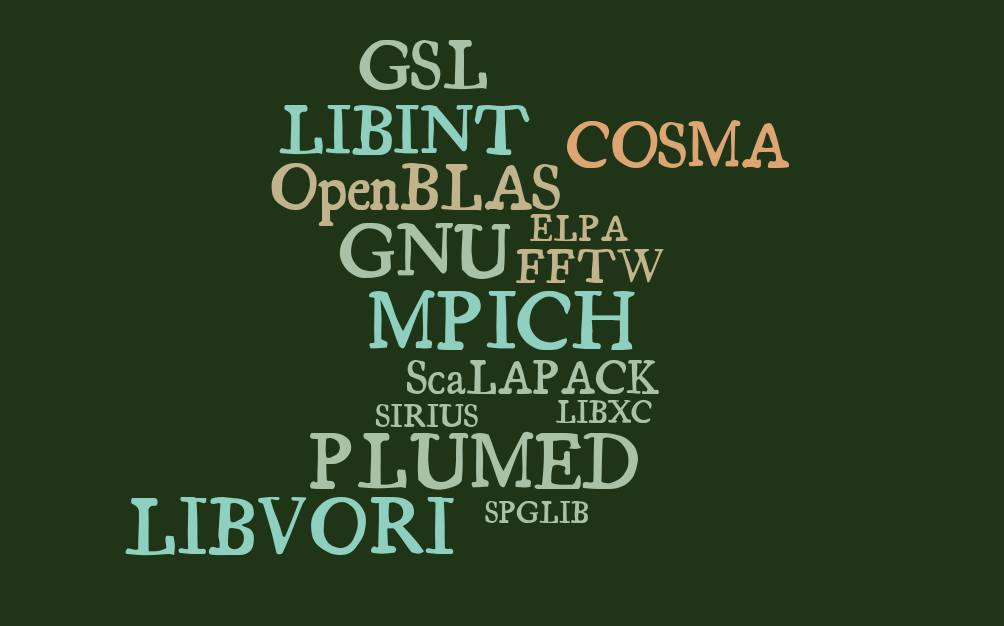
\includegraphics[width=0.7\linewidth]{fig/cp2k-lib.jpg}
    \caption{ไลบรารี่ที่โปรแกรม CP2K ใช้ในการช่วยคำนวณ}
    \label{fig:cp2k_lib}
\end{figure}

ผมจะมาอธิบายบาง Library ที่สำคัญ ๆ ของ CP2K ใช้ ดังนี้

\begin{description}
    \item[GNU] แน่นอนว่าเราต้องคอมไพล์ Source Code ดังนั้นเราจะต้องใช้ตัวคอมไพล์ (Compiler) ซึ่ง CP2K เลือกใช้ GNU เป็น Compiler
    
    \item[OpenBLAS กับ ScaLAPACK]  สำหรับ Linear Algebraic Calculation เช่น Matrix-vector, Matrix-matrix Multiplication 
    
    \item[MPICH] อยากจะรันโปรแกรมแบบขนานโดยใช้ MPI ก็ต้องหา Implementation ที่จะมารันโค้ดของเรา ซึ่ง MPICH ก็เป็นหนึ่งใน
    Implementation ของ MPI ที่ CP2K เลือกใช้
    
    \item[FFTW] สำหรับทำฟูเรียร์ทรานฟอร์มในการคำนวณ DFT หรือแปลงจาก Real Space ไปเป็น Reciprocal Space สำหรับการคำนวณ 
    Electrostatics โดยใช้ Plane Wave Electron Density
    
    \item[LIBXC] เป็น Library ที่ให้เราสามารถนำ DFT Functional มาใช้ได้เลยโดยไม่ต้อง Implement เอง
\end{description}

สรุปก็คือจะเห็นได้ว่าการเขียนโค้ดของโปรแกรมเคมีควอนตัมนั้นมีความซับซ้อนมากดังนั้นเรามีสองทางเลือกคือ 

\begin{enumerate}
    \item ใช้ Library ที่มีอยู่แล้วสำหรับการทำงานเฉพาะจุด
    
    \item เขียนโค้ดทั้งหมดเองเลย
\end{enumerate}

แน่นอนว่าถ้าเราเลือกวิธีแรกก็จะประหยัดเวลาไปได้เยอะมากและเวลาที่เราคอมไพล์โปรแกรมก็ขอแค่ Link กับ Library ต่าง ๆ ก็รันโปรแกรมได้แล้ว%
และทำให้ขนาดของตัวโปรแกรมของเรา (ขนาดของ Binary Files) นั้นมีขนาดไม่ใหญ่มากเกินไปด้วย (เช่นหลักสิบ-ร้อยเมกะไบต์) 

อย่างไรก็ตามโปรแกรมสำหรับจำลองระบบโมเลกุลหลาย ๆ โปรแกรมก็ไม่ได้ใช้ Library เหล่านี้และเลือกใช้วิธีที่ 2 ก็คือการเขียนโค้ดสำหรับการ%
คำนวณส่วนต่าง ๆ เองเลยเนื่องด้วยเหตุหลายข้อ เช่น การเขียนโค้ดทั้งหมดภายใน Framework โปรแกรมเดียวกันนั้นจะทำให้โค้ดมีประสิทธิภาพและ%
ทำงานร่วมกันได้ดี (Compatibility), ง่ายต่อการดูแลรักษาและปรับปรุงโค้ดเพราะว่า Developers นั้นรู้และเข้าใจการทำงานของโค้ดทั้งหมด, 
ถึงแม้ว่าโปรแกรมที่เขียนโค้ดทั้งหมดเองเมื่อถูกคอมไพล์แล้วจะได้ออกมาเป็น Binary File ที่มีขนาดนั้นใหญ่มาก ๆ เช่น หลายกิกะไบต์ แต่ว่าก็มี%
ความคล่องตัวในการใช้งานเพราะว่าไม่ต้องติดตั้ง Library อื่น ๆ เพิ่มเติม 

นอกจากนี้แล้วการที่ใช้ Library หลาย ๆ ตัวแบบนี้ก็มีจุดอ่อนบางข้อที่เราควรจะต้องรู้ไว้นั่นก็คือการเข้ากันได้ (Compatibility) ระหว่าง Library 
หรือเวอร์ชันซึ่งก็อาจจะทำให้เราปวดหัวได้ถ้าหากว่า Library บางตัวมีการอัพเดทเวอร์ชันใหม่แล้ว Conflict กับ Library ตัวอื่น

%----------------------------------------
\section{แบบฝึกหัด}
%----------------------------------------
